
\section{Materiais e Métodos}
\label{sec:materiais}

Esta seção apresenta os procedimentos metodológicos adotados para a condução da pesquisa, bem como os instrumentos utilizados para coleta e análise dos dados. A pesquisa caracteriza-se como um estudo empírico, quantitativo e comparativo, cujo objetivo é investigar se a inclusão do código influencia a avaliação da qualidade de descrições de ferramentas MCP.


O fluxo metodológico adotado encontra-se resumido na Figura \ref{fig:metodologia}. O processo inicia-se com a coleta de repositórios MCP públicos, seguida pela extração das ferramentas e das informações sobre sua implementação. Em seguida, a qualidade das descrições das ferramentas é avaliada em dois cenários distintos: no primeiro, considerando a descrição em linguagem natural da ferramenta; no segundo, considerando a mesma descrição acompanhada pelo código correspondente. Por fim, os resultados obtidos são organizados e submetidos a uma análise comparativa e estatística.

\begin{figure}[H]
    \centering
    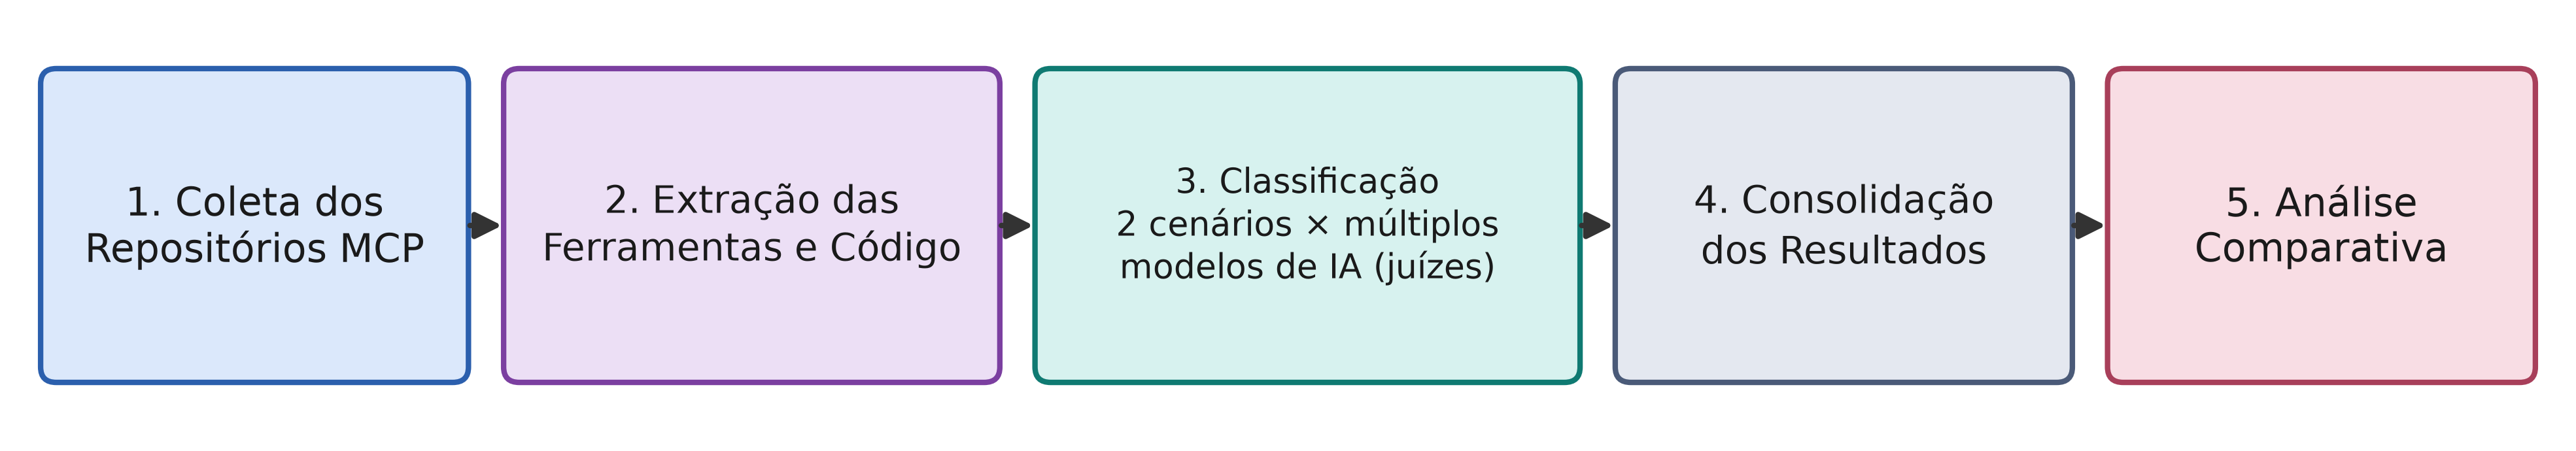
\includegraphics[width=1\linewidth]{./images/metodologia_v7.png}
    \caption{Fluxo metodológico adotado na pesquisa}
    \label{fig:metodologia}
\end{figure}

\subsection{Coleta dos Repositórios MCP}

A primeira etapa consiste na construção do conjunto de dados que servirá de base para os experimentos. Para isso, foram minerados repositórios públicos relacionados ao ecossistema MCP hospedados no GitHub. O objetivo dessa etapa é identificar implementações reais de servidores MCP que representem o cenário atual.

\textcolor{blue} {As consultas foram construídas a partir dos nomes dos pacotes necessários para a implementação do MCP. Para cada pacote, seu nome foi utilizado como termo de busca nos arquivos de dependências dos projetos. Essa etapa foi realizada por meio da busca de código da API REST do GitHub, que permite localizar repositórios com base em termos presentes no conteúdo de seus arquivos, ainda que a API limite cada consulta a um máximo de 1.000 resultados \cite{BashInTheWild}. Dessa forma, foi necessário dividir a busca em consultas distintas, a fim de ampliar a quantidade de projetos identificáveis. Para isso, foi realizada uma consulta para cada combinação entre o nome da dependência e o respectivo arquivo de dependências em que ela poderia estar declarada. Como essa busca de código não devolve metadados do repositório em si, cada resultado foi complementado por uma consulta separada à API GraphQL do GitHub, de onde vieram o número de estrelas, a condição de \textit{fork} e a linguagem principal usados nos filtros seguintes. Ao final, os repositórios duplicados foram unificados por identificador. Após isto, os que eram \textit{fork} e os que não atingiam o piso mínimo de estrelas, ou cuja linguagem principal não estava entre as linguagens-alvo do estudo, foram removidos.}

Para garantir a relevância e a maturidade dos \textit{softwares} analisados, a coleta foi restrita a repositórios que possuam no mínimo 100 estrelas (\textit{stars}). A adoção desse limiar fundamenta-se em estudos de mineração de repositórios que identificam o número de estrelas como uma medida direta de popularidade, sendo 100 estrelas um marco estatístico comum para filtrar projetos experimentais ou de baixo valor agregado, conhecidos como \textit{toy repositories} \cite{Borges2016}. Ao final, foram selecionados os 206 servidores mais populares encontrados e que possuíam ao menos uma tool, dobrando a amostra utilizada no estudo de Hasan et al. (2026)\nocite{2026arXiv260214878M} para ampliar a cobertura do ecossistema investigado.


\subsection{Extração das Ferramentas e do Código Relacionado}

Após a obtenção dos repositórios, cada um foi clonado localmente   para permitir a identificação automática das ferramentas
disponibilizadas por cada servidor MCP, chegando ao resultado de 12.171
ferramentas. Para isso, foi desenvolvido um algoritmo de mineração capaz
de percorrer a estrutura dos projetos e localizar as implementações
associadas às ferramentas expostas pelo servidor. Para cada ferramenta
identificada, foram extraídos sua descrição em linguagem natural e sua
localização no código. Um repositório em que nenhuma ferramenta é
localizada é tratado, na prática, como um falso positivo da etapa de
coleta: ele é removido da amostra e substituído pelo próximo candidato
ainda não testado, repetindo-se o processo até completar o número de
repositórios definido para o estudo ou esgotar os candidatos disponíveis
(Seção~\ref{sec:resultados}).

Em seguida, foi realizada a extração do código relacionado a cada ferramenta. Como os servidores MCP possuem estruturas variadas, extrair apenas o método raiz de uma ferramenta pode não ser suficiente para capturar sua lógica, sendo necessário incluir também os métodos subsequentemente invocados. Para isso, foi construída uma árvore de chamadas (\textit{call graph}) composta por três níveis a partir do método inicial: o próprio método inicial constitui o primeiro nível; os métodos chamados diretamente por ele formam o segundo nível; e as chamadas efetuadas a partir destes compõem o terceiro nível. A limitação da análise estática até essa profundidade apoia-se em evidências empíricas da literatura, que demonstram que esse limite captura a vasta maioria da lógica de negócios local da ferramenta, enquanto níveis adicionais introduzem predominantemente ruído advindo de bibliotecas externas \cite{shi2026description}. Um exemplo desse processo é apresentado na Figura \ref{fig:codigoarvore}.

\begin{figure}[H]
    \centering
    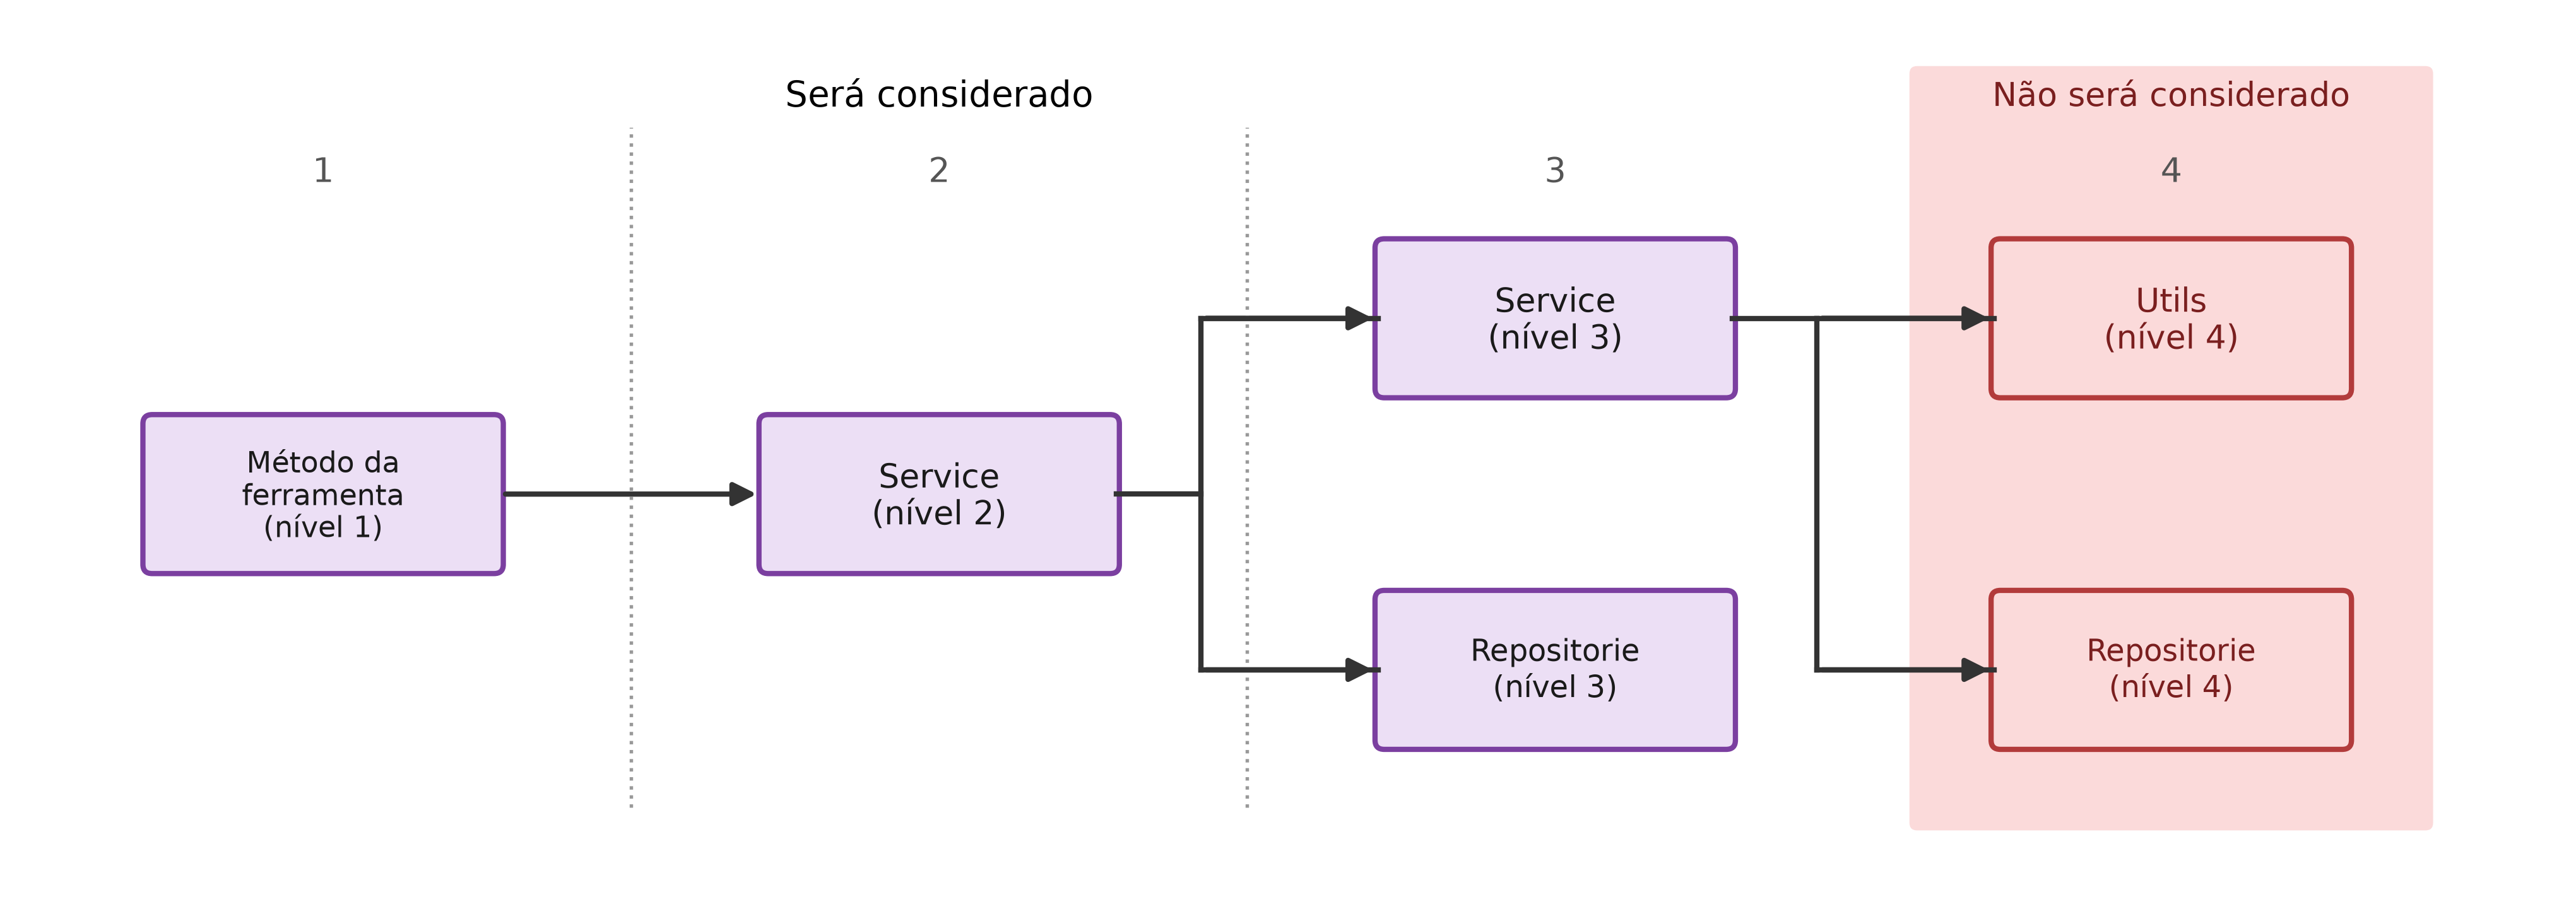
\includegraphics[width=1\linewidth]{./images/arvoreFinal.png}
    \caption{Exemplo de extração da árvore de chamadas de uma ferramenta}
    \label{fig:codigoarvore}
\end{figure}

Ao final desta etapa, foi produzido um conjunto de dados estruturado contendo os servidores MCP analisados e as ferramentas identificadas em cada um deles. Para cada ferramenta, serão armazenadas sua descrição em linguagem natural e o conjunto de métodos obtido a partir da árvore de chamadas. Esse conjunto de dados servirá como entrada para as etapas subsequentes da pesquisa, nas quais as ferramentas dos repositórios coletados serão avaliadas quanto à qualidade de suas descrições, com e sem o uso do código correspondente.

\subsection{Classificação das tools por diferentes modelos de IA}

Na terceira etapa, utilizando as \textit{tools} coletadas nas etapas anteriores, será conduzido um experimento comparativo estruturado em dois cenários de avaliação que serão executados em diferentes modelos de IA . No primeiro cenário, as descrições das ferramentas serão avaliadas com base em seu conteúdo em linguagem natural. No segundo, essas mesmas descrições serão avaliadas em conjunto com informações extraídas do código correspondente. Essa estratégia permite identificar o impacto da inclusão do contexto de implementação na avaliação da qualidade das descrições.

Em ambos os cenários, a avaliação será conduzida com base na rubrica proposta por Hasan et al. (2026)\nocite{2026arXiv260214878M}, composta por seis componentes: \textit{Purpose}, que avalia a clareza com que a descrição comunica a finalidade da ferramenta; \textit{Guidelines}, que verifica se existem orientações sobre quando e como utilizá-la; \textit{Limitations}, que analisa a explicitação de restrições, premissas ou casos de falha; \textit{Parameter Explanation}, que mede a qualidade da documentação dos parâmetros de entrada; \textit{Length and Completeness}, que avalia o nível de detalhamento e cobertura da descrição; e \textit{Examples}, que verifica a presença de exemplos de utilização. Cada componente recebe uma pontuação em uma escala Likert de cinco pontos, sendo posteriormente utilizada para identificar deficiências associadas aos respectivos \textit{smells} descritos pelos autores.

No primeiro cenário, os modelos de linguagem atuarão como avaliadores (\textit{LLM-as-a-Judge}) recebendo as descrições das ferramentas. Nesse contexto, a classificação será realizada sem qualquer acesso à implementação da funcionalidade analisada. No segundo cenário, além da descrição da ferramenta, o modelo receberá também o código correspondente. Dessa forma, o avaliador poderá confrontar a descrição fornecida com aspectos observáveis da implementação, verificando a existência de omissões, inconsistências ou informações potencialmente enganosas que não seriam perceptíveis apenas pela análise da descrição.


\subsection{Coleta e Organização dos Resultados}

Concluída a etapa de classificação, os resultados produzidos nos dois cenários experimentais serão coletados e estruturados em uma base de dados unificada. Para cada ferramenta analisada, serão armazenados identificadores que permitam sua associação ao servidor MCP de origem, bem como os resultados obtidos nos cenários com e sem a inclusão de informações provenientes do código, além de qual modelo de IA foi utilizado para a analise.

A base de dados resultante conterá os escores atribuídos pelo modelo para cada dimensão de qualidade avaliada, além das classificações finais produzidas em cada execução do experimento. Dessa forma, cada ferramenta possuirá dois conjuntos de resultados por modelo que estarão diretamente vinculados à mesma descrição, diferindo apenas pela presença ou ausência das informações extraídas do código. Essa organização permitirá estabelecer um relacionamento direto entre as avaliações realizadas sobre uma mesma ferramenta, preservando o pareamento necessário para as análises estatísticas subsequentes e possibilitando a comparação consistente dos resultados obtidos nos dois cenários experimentais.

\subsection{Análise Comparativa dos Experimentos}

Na etapa final, os resultados obtidos serão analisados com o objetivo de identificar diferenças entre os dois cenários de avaliação. Essa análise busca validar se a utilização do código de fato altera os resultados da avaliação das descrições, além de identificar quais atributos da rubrica utilizada para avaliar a qualidade são mais e menos impactados pela adição do código.

Inicialmente, será realizada uma análise por meio do cálculo de medidas como média, mediana e desvio-padrão dos escores atribuídos a cada dimensão de qualidade avaliada, para identificar se houve diferença numérica nos resultados gerados com e sem o contexto do código das ferramentas MCP, atendendo ao objetivo específico (ii) desta pesquisa. A partir dessa comparação, será possível avaliar quais atributos foram mais afetados pela inserção do contexto técnico. Será realizado também o Teste de Postos Sinalizados de Wilcoxon \cite{wilcoxon1945individual}, aplicado individualmente para cada dimensão de qualidade, a fim de verificar se as diferenças observadas entre as avaliações são estatisticamente significativas, concluindo o objetivo específico (iii). O teste será aplicado separadamente para cada modelo de linguagem utilizado, permitindo verificar se o efeito da inclusão do código se mantém consistente entre diferentes avaliadores. Como as duas avaliações são realizadas sobre a mesma ferramenta, o teste é adequado por considerar amostras pareadas e não exigir a suposição de normalidade dos dados. Os resultados dessa análise fornecerão as evidências empíricas necessárias para apoiar ou refutar a hipótese de que a incorporação do contexto técnico amplia a capacidade de detecção de \textit{smells} em descrições de ferramentas MCP.
